\documentclass[conference]{IEEEtran}
\usepackage[utf8]{inputenc}
\usepackage[T5]{fontenc}
\usepackage{cite}
\usepackage{amsmath,amssymb}
\usepackage{graphicx}
\usepackage{booktabs,array}
\usepackage{url}
\usepackage[hidelinks]{hyperref}
\graphicspath{{BaoCao/image_result/}}
\newcommand{\CE}{\operatorname{CE}}
\newcommand{\KL}{\operatorname{KL}}
% Fixed type size for all tables; fit columns without scaling the text.
\newcommand{\reporttablefont}{\normalfont\small}

\renewcommand{\figurename}{Hình}
\renewcommand{\tablename}{Bảng}
\renewcommand{\refname}{Tài liệu tham khảo}
\begin{document}
\title{Đánh giá Boundary Unlearning trên CIFAR-10 và CIFAR-100}
\author{\IEEEauthorblockN{Nguyễn Viết Hòa, Nguyễn Quang Khải, Nguyễn Tiến Nhật}
\IEEEauthorblockA{Khoa Toán - Tin\\
Đại học Khoa học Tự nhiên\\
Đại học Quốc gia Thành phố Hồ Chí Minh}}
\maketitle
\begin{abstract}
Machine Unlearning hướng đến loại bỏ ảnh hưởng của dữ liệu được yêu cầu quên khỏi mô hình đã huấn luyện. Tuy nhiên, huấn luyện lại mô hình từ đầu trên phần dữ liệu còn lại thường tốn nhiều thời gian và tài nguyên. Boundary Unlearning tiếp cận vấn đề này bằng cách dịch chuyển ranh giới quyết định, nhằm thay đổi dự đoán trên lớp cần quên trong khi hạn chế ảnh hưởng đến các lớp cần giữ lại. Nghiên cứu này đánh giá hai phương pháp Boundary Shrink và Boundary Expanding, đồng thời khảo sát các cấu hình cải tiến của Boundary Shrink thông qua tìm ngưỡng vượt biên, gán trọng số theo độ tin cậy của nhãn giả và chưng cất tri thức với mô hình đã được huấn luyện trước. Các thí nghiệm so sánh phương pháp với mô hình Original và Retrain trên CIFAR-10 và CIFAR-100, riêng các cấu hình cải tiến được đánh giá trên CIFAR-10. Kết quả cho thấy Boundary Shrink và Boundary Expanding giảm khả năng nhận diện lớp cần quên, nhưng làm suy giảm hiệu năng trên các lớp cần giữ lại. Các cấu hình cải tiến khôi phục một phần hiệu năng trên lớp giữ lại, đi kèm với chi phí tính toán cao hơn.
\end{abstract}
\begin{IEEEkeywords}
Machine Unlearning, Class Unlearning, Boundary Shrink, Boundary Expanding, CIFAR-10, CIFAR-100, Knowledge Distillation.
\end{IEEEkeywords}

\section{Giới thiệu}
Trong bối cảnh dữ liệu ngày càng được khai thác rộng rãi để huấn luyện các mô hình học máy, nhu cầu loại bỏ dữ liệu khỏi các mô hình đã được huấn luyện cũng ngày càng được quan tâm. Tuy nhiên, việc xóa dữ liệu khỏi kho lưu trữ chưa thể loại bỏ những ảnh hưởng của dữ liệu đó trong mạng nơ-ron đã huấn luyện. Để giải quyết vấn đề này, Machine Unlearning nghiên cứu các phương pháp cập nhật mô hình nhằm giảm thiểu ảnh hưởng của những dữ liệu được yêu cầu gỡ bỏ, đồng thời đáp ứng các yêu cầu về quản trị dữ liệu và quyền riêng tư~\cite{bourtoule2021machine}. Một phương pháp đối chứng thường được sử dụng là huấn luyện lại mô hình từ đầu trên tập dữ liệu đã loại bỏ các mẫu cần quên. Phương pháp này cung cấp cơ sở so sánh, tuy nhiên đòi hỏi tài nguyên tính toán và thời gian huấn luyện đáng kể. Hiệu quả của một kỹ thuật Machine Unlearning được xem xét trên ba khía cạnh chính: mức độ giảm thiểu ảnh hưởng của dữ liệu cần quên, khả năng duy trì hiệu năng của mô hình trên dữ liệu còn lại và chi phí tính toán trong quá trình thực hiện.

Boundary Unlearning của Chen và cộng sự~\cite{chen2023boundary} điều chỉnh ranh giới quyết định thông qua hai cơ chế Boundary Shrink và Boundary Expanding. Chúng tôi kế thừa hai phương pháp này và cải tiến Boundary Shrink bằng phương pháp Weight Assign, sau đó tiến hành so sánh và đánh giá hiệu quả của các phương pháp với nhau.

Phạm vi gồm hai phần: so sánh cùng bốn mô hình Original, Retrain, Boundary Shrink và Boundary Expanding trên CIFAR-10 và CIFAR-100; sau đó khảo sát hai biến thể cải tiến của Boundary Shrink chỉ trên CIFAR-10. Nghiên cứu tập trung đánh giá mức giảm accuracy lớp quên và mức suy giảm trên các lớp giữ lại so với Retrain, đồng thời đối chiếu chi phí trong hai thiết lập có quy mô tập quên khác nhau. Riêng trên CIFAR-10, chúng tôi khảo sát liệu hai biến thể có cải thiện đánh đổi giữa accuracy giữ lại, accuracy lớp quên và thời gian thực hiện hay không.

Đóng góp của đồ án là tổ chức so sánh trên hai dataset, triển khai và khảo sát hai biến thể của Boundary Shrink trên CIFAR-10, cùng phân tích đánh đổi giữa hiệu năng và chi phí.

\section{Các nghiên cứu liên quan}
SISA~\cite{bourtoule2021machine} tổ chức huấn luyện thành các phân mảnh để giới hạn ảnh hưởng của mẫu và giảm phần cần học lại khi xóa. Cách tiếp cận này yêu cầu tổ chức phân mảnh dữ liệu ngay từ giai đoạn huấn luyện ban đầu. Một hướng khác điều chỉnh trọng số mô hình đã học, chẳng hạn selective forgetting~\cite{golatkar2020eternal}. Chi phí và chất lượng của các phương pháp phụ thuộc vào phép xấp xỉ và thiết lập thực nghiệm.

Boundary Unlearning~\cite{chen2023boundary} dùng trực giác về ranh giới quyết định để thiết kế cập nhật. Quan sát trực quan cung cấp động lực cho thuật toán, còn chất lượng quên được lượng hóa thông qua đối chiếu với Retrain. Báo cáo tập trung đánh giá hai cơ chế Boundary Shrink và Boundary Expanding trong cùng quy trình thực nghiệm.

Các thành phần kế thừa gồm FGSM~\cite{goodfellow2015explaining}, AllCNN~\cite{springenberg2015allcnn} với Batch Normalization~\cite{ioffe2015batch} và chưng cất tri thức~\cite{hinton2015distilling}. Grad-CAM~\cite{selvaraju2017gradcam} và t-SNE~\cite{maaten2008tsne} bổ sung phân tích định tính về hành vi của các mô hình sau unlearning.
\section{Phương pháp}

Với tập train $D$, tập cần quên $D_f$ chứa toàn bộ mẫu của một lớp và tập giữ lại là $D_r=D\setminus D_f$. Ký hiệu $D_{ft},D_{rt}$ là các tập test tương ứng. Original ($f_{w_0}$) được học trên $D$; Retrain ($f_{w^*}$) học từ đầu trên $D_r$. Cả hai giữ $K$ đầu ra. Hai cơ chế kế thừa để cập nhật Original là Boundary Shrink và Boundary Expanding~\cite{chen2023boundary}.

\begin{figure}[!b]
\centering
\includegraphics[width=\linewidth]{\detokenize{paper_fig2_boundary_shrink_expanding.png}}
\caption{Nguyên lý Boundary Shrink và Boundary Expanding, trích từ Chen và cộng sự~\cite{chen2023boundary}.}
\label{fig:boundary-methods}
\end{figure}

\subsection{Phương pháp Boundary Shrink}
Việc gán nhãn ngẫu nhiên cho các mẫu thuộc $D_f$ rồi tiếp tục huấn luyện có thể làm biến dạng ranh giới của các lớp giữ lại lân cận. Để khắc phục điều này, Boundary Shrink sử dụng kỹ thuật tìm kiếm lân cận (Neighbor Searching) dựa trên hướng gradient đối kháng.

Với mỗi mẫu cần quên $x_f \in D_f$ có nhãn gốc $y$, mẫu biến dạng $x'_f$ được sinh ra theo hướng tăng của hàm mất mát phân loại từ mô hình gốc $f_{w_0}$:
\begin{equation}
x'_f = x_f + \epsilon \cdot \operatorname{sign}\!\left(\nabla_{x_f} \mathcal{L}(x_f,y,w_0)\right).
\end{equation}
Trong triển khai, nhiễu được xử lý trong miền pixel, chặn vào $[0,1]$, làm tròn 8-bit rồi chuẩn hóa trước khi đưa vào mạng. Với $\epsilon$ cố định, khả năng vượt biên phụ thuộc vào từng mẫu.

Mẫu $x'_f$ sau đó được đưa qua mô hình gốc $f_{w_0}$ để thu nhận nhãn dự đoán mới:
\begin{equation}
y_{nbi} \leftarrow \arg\max_k \operatorname{softmax}\!\left(f_{w_0}(x'_f)\right).
\end{equation}
Nhãn thu được phụ thuộc vào hướng và độ lớn nhiễu, có thể trùng với nhãn gốc. Tỷ lệ vượt biên được xác định bằng tỷ lệ mẫu có nhãn dự đoán mới khác nhãn gốc.

Mô hình được tinh chỉnh bằng các mẫu ảnh gốc $x_f$ kết hợp với nhãn mục tiêu mới $y_{nbi}$:
\begin{equation}
w' = \arg\min_w \frac{1}{|D_f|}\sum_{(x_i,y_i)\in D_f} \CE(f_w(x_i),\widetilde y_i),
\end{equation}
trong đó $\widetilde y_i=y_{nbi}(x_i)$ là nhãn mục tiêu đã tạo cho từng ảnh. Quá trình cập nhật nhằm thay đổi dự đoán trên lớp quên theo các nhãn này.

\subsection{Phương pháp Boundary Expanding}
Nhằm giảm bớt thời gian tính toán gradient khi tạo mẫu xuyên biên trong Boundary Shrink, cơ chế Boundary Expanding mở rộng không gian lớp bằng cách bổ sung một nơ-ron vào tầng phân loại cuối cùng, nâng số chiều đầu ra từ $K$ lên $K+1$. Nơ-ron bổ sung đóng vai trò là lớp bóng (Shadow Class), ký hiệu $y_{shadow}$.

Mô hình mở rộng được tinh chỉnh trên tập dữ liệu quên $D_f$ với nhãn mục tiêu là $y_{shadow}$:
\begin{equation}
w'=\arg\min_w\frac{1}{|D_f|}\sum_{(x_i,y_i)\in D_f}\CE(f_w(x_i),y_{shadow}).
\end{equation}
Thao tác này chuyển hướng các kích hoạt liên quan đến $D_f$ về nơ-ron phụ, làm suy giảm đáp ứng của nơ-ron đại diện cho lớp quên ban đầu.

Sau một số epoch tinh chỉnh ngắn, nơ-ron thứ $K+1$ được loại bỏ khỏi mạng, đưa mô hình về $K$ đầu ra. Dự đoán sau cắt tỉa được xác định từ các logit của những đầu ra còn lại.


\subsection{Boundary Shrink with weight assign}

Nhận thấy Boundary Shrink dùng nhãn giả để tinh chỉnh trên ảnh gốc, nhưng mô hình tinh chỉnh không được biết mức độ tin cậy của các nhãn giả. Nếu xác suất của lớp được chọn chỉ nhỉnh hơn lớp đứng thứ hai một chút, chứng tỏ mô hình còn phân vân giữa hai lớp và mẫu có thể nằm gần ranh giới quyết định.

Do đó, Weight Assign dùng khoảng cách giữa hai xác suất này để gán trọng số tương đối lớn hơn cho những mẫu mơ hồ, nhỏ hơn cho những mẫu mô hình đã có độ tin cậy cao. Nhờ đó, quá trình tinh chỉnh ưu tiên tương đối nhiều hơn các mẫu mà mô hình còn phân vân.

Trong biến thể \textit{Weight Assignment}, mô hình gốc cố định \(f_{\theta_0}\) dự đoán trên ảnh đã làm nhiễu \(x'_f\), tạo phân phối xác suất:

\[
p_i = \operatorname{softmax}(f_{\theta_0}(x'_f))
\]

và nhãn giả:

\[
\hat{y}_i = \arg\max_c p_{i,c}.
\]

Gọi \(p_i^{(1)} = p_{i,\hat{y}_i}\) là xác suất cao nhất và \(p_i^{(2)} = \max_{c\ne\hat{y}_i}p_{i,c}\) là xác suất cao thứ hai. Độ chênh:

\[
PM_i = p_i^{(2)} - p_i^{(1)}
\]

được dùng để tính trọng số:

\[
w_i = 3\sigma\!\left(5(PM_i-0.5)\right),
\]

trong đó \(\sigma\) là hàm sigmoid.

Khi hai xác suất gần nhau, nhãn giả kém chắc chắn và mẫu nhận trọng số tương đối lớn hơn.

Mô hình đang tinh chỉnh \(f_\theta\) được huấn luyện trên ảnh gốc \(x_i\) bằng loss:

\[
\mathcal{L}_{\mathrm{WA}}(\theta)
=
\frac{1}{B}
\sum_{i=1}^{B}
w_i\,\operatorname{CE}(f_\theta(x_i),\hat{y}_i).
\]

Ảnh nhiễu chỉ dùng để xác định nhãn giả và trọng số.

Với cấu hình trọng số trên, mọi \(w_i\) đều nhỏ hơn \(1\), nên mẫu kém chắc chắn được giảm trọng số ít hơn mẫu chắc chắn.
\section{Thiết lập thực nghiệm}
\label{sec:protocol}
\subsection{Dữ liệu và cấu hình thực nghiệm}
Tập dữ liệu CIFAR-10~\cite{krizhevsky2009learning} gồm 50.000 ảnh huấn luyện và 10.000 ảnh kiểm thử thuộc 10 lớp đối tượng, kích thước $32\times32\times3$. Lớp cần quên được chọn là lớp số 4 (\texttt{deer}). Tập $D_f$ gồm 5.000 ảnh huấn luyện của lớp này; tập $D_r$ gồm 45.000 ảnh thuộc 9 lớp còn lại. Tập kiểm thử gồm 1.000 ảnh lớp quên ($D_{ft}$) và 9.000 ảnh thuộc các lớp giữ lại ($D_{rt}$).

CIFAR-100~\cite{krizhevsky2009learning} có cùng kích thước ảnh và số lượng ảnh huấn luyện, kiểm thử như CIFAR-10, với 100 lớp theo nhãn chi tiết (fine labels). Lớp cần quên là lớp số 4 (\texttt{beaver}), gồm 500 ảnh huấn luyện và 100 ảnh kiểm thử. Tập giữ lại gồm 49.500 ảnh huấn luyện và 9.900 ảnh kiểm thử thuộc 99 lớp còn lại.

Hai thiết lập sử dụng AllCNN~\cite{springenberg2015allcnn} với hệ số số kênh 0.5, gồm tám lớp tích chập kết hợp BatchNorm và ReLU, average pooling và bộ phân loại tuyến tính. Số đầu ra tương ứng là 10 và 100; tổng số tham số lần lượt là 406.810 và 415.540. Ảnh đầu vào được chuẩn hóa theo từng kênh với trung bình $\mu=(0.5,0.5,0.5)$ và độ lệch chuẩn $\sigma=(0.5,0.5,0.5)$. Các thí nghiệm dùng seed 2022.

Original và Retrain được huấn luyện trong 30 epoch bằng SGD với tốc độ học $\eta=0.1$, hệ số động lượng $0.9$ và kích thước mini-batch 64. Original được huấn luyện trên toàn bộ 50.000 ảnh của từng dataset. Retrain được huấn luyện lại từ đầu trên $D_r$, tương ứng 45.000 ảnh CIFAR-10 hoặc 49.500 ảnh CIFAR-100, đồng thời giữ nguyên số đầu ra.

Boundary Shrink và Boundary Expanding thực hiện 10 epoch unlearning với SGD, tốc độ học $\eta=10^{-5}$, hệ số động lượng $0.9$ và batch size 64. Số bước cập nhật được tính bằng $10\lceil|D_f|/64\rceil$, tương ứng 790 bước trên CIFAR-10 và 80 bước trên CIFAR-100. Boundary Shrink sử dụng ngưỡng nhiễu 0.1, không khởi tạo nhiễu ngẫu nhiên.

Trong bước tạo nhiễu của Boundary Shrink trên CIFAR-10, các hệ số chuẩn hóa là $\mu_a=(0.4914,0.4822,0.2265)$ và $\sigma_a=(0.2023,0.1994,0.2010)$. Trên CIFAR-100, bước tạo nhiễu sử dụng cùng các hệ số chuẩn hóa với ảnh đầu vào.

\subsection{Các tiêu chí đánh giá}
Tính hữu ích (Utility) được lượng hóa bằng độ chính xác trên tập giữ lại trong huấn luyện $\operatorname{Acc}(D_r)$ và kiểm thử $\operatorname{Acc}(D_{rt})$. Mức độ nhận diện lớp quên được lượng hóa tương ứng bằng $\operatorname{Acc}(D_f)$ và $\operatorname{Acc}(D_{ft})$. Retrain là mốc đối chiếu cho cả bốn chỉ số; độ chính xác test-retain phản ánh khả năng tổng quát hóa trên các lớp giữ lại.

Hiệu quả tính toán (Computational Efficiency) được đo bằng thời gian thực hiện, tính bằng giây. Thời gian huấn luyện được ghi nhận cho Original và Retrain; thời gian unlearning được ghi nhận cho Boundary Shrink, Boundary Expanding và các biến thể. Hệ số tăng tốc là tỷ số giữa thời gian huấn luyện Retrain và thời gian unlearning trong cùng thiết lập. Với DW+KL-S, tổng thời gian và tổng số bước cập nhật bao gồm việc tạo mô hình DW dùng khởi tạo student và mô hình Boundary Shrink dùng làm teacher; các chi phí này không bao gồm huấn luyện Original dùng chung.

Khả năng giải thích (Explainability) được khảo sát thông qua bản đồ Grad-CAM trên các mẫu của lớp quên và trực quan hóa phân bố biểu diễn trong không gian đặc trưng bằng t-SNE. ECDF entropy bổ sung mô tả độ bất định của phân phối đầu ra.

\section{Kết quả thực nghiệm}
\subsection{Bốn mô hình cơ sở trên hai dataset}
\begin{table}[t]
\centering
\caption{Độ chính xác (\%) của các mô hình cơ sở trên CIFAR-10 và CIFAR-100.}
\label{tab:baseline}
\reporttablefont
\setlength{\tabcolsep}{1.5pt}
\renewcommand{\arraystretch}{1.08}
\begin{tabular*}{\columnwidth}{@{\extracolsep{\fill}}>{\raggedright\arraybackslash}p{0.63in}>{\raggedright\arraybackslash}p{0.84in}*{5}{c}@{}}
\toprule
Dataset & Mô hình & \shortstack{Train\\ret.} & \shortstack{Train\\forg.} & \shortstack{Test\\ret.} & \shortstack{Test\\forg.} & \shortstack{Test\\all} \\
\midrule
CIFAR-10 & Original & 99.43 & 99.64 & 73.46 & 68.00 & 72.91\\
& Retrain & 99.70 & 0.00 & 75.61 & 0.00 & 68.05\\
& Boundary Shrink & 94.86 & 11.54 & 62.07 & 2.30 & 56.09\\
& Boundary Expanding & 94.95 & 11.34 & 62.57 & 2.20 & 56.53\\
\midrule
CIFAR-100 & Original & 95.30 & 95.40 & 52.65 & 26.00 & 52.38\\
& Retrain & 95.62 & 0.00 & 52.27 & 0.00 & 51.75\\
& Boundary Shrink & 72.98 & 0.00 & 43.42 & 0.00 & 42.99\\
& Boundary Expanding & 72.96 & 0.00 & 43.39 & 0.00 & 42.96\\
\bottomrule
\end{tabular*}
\end{table}
Bảng~\ref{tab:baseline} trình bày kết quả của bốn mô hình cơ sở. Trên CIFAR-10, Boundary Shrink và Boundary Expanding giảm test-forget từ 68.00\% của Original xuống 2.30\% và 2.20\%, nhưng test-retain còn 62.07\% và 62.57\%, thấp hơn Retrain 13.54 và 13.04 điểm phần trăm. Train-forget vẫn đạt 11.54\% và 11.34\%, trong khi Retrain đạt 0\%. Hai phương pháp giảm mạnh khả năng nhận diện lớp quên nhưng chưa đạt hành vi tương đương Retrain theo các độ đo này.

CIFAR-100: cả hai có train/test-forget 0\%, nhưng test-retain 43.42\% và 43.39\%, thấp hơn Retrain 8.85 và 8.88 điểm. Train-retain giảm từ 95.62\% của Retrain xuống khoảng 72.97\%. Kết quả cho thấy giảm khả năng nhận diện lớp quên đi kèm suy giảm hiệu năng trên các lớp giữ lại. Hai thiết lập khác nhau về số mẫu forget, số bước cập nhật và chuẩn hóa attack; chênh lệch giữa hai dataset phản ánh ảnh hưởng kết hợp của các yếu tố này.

\begin{figure*}[!t]
\centering
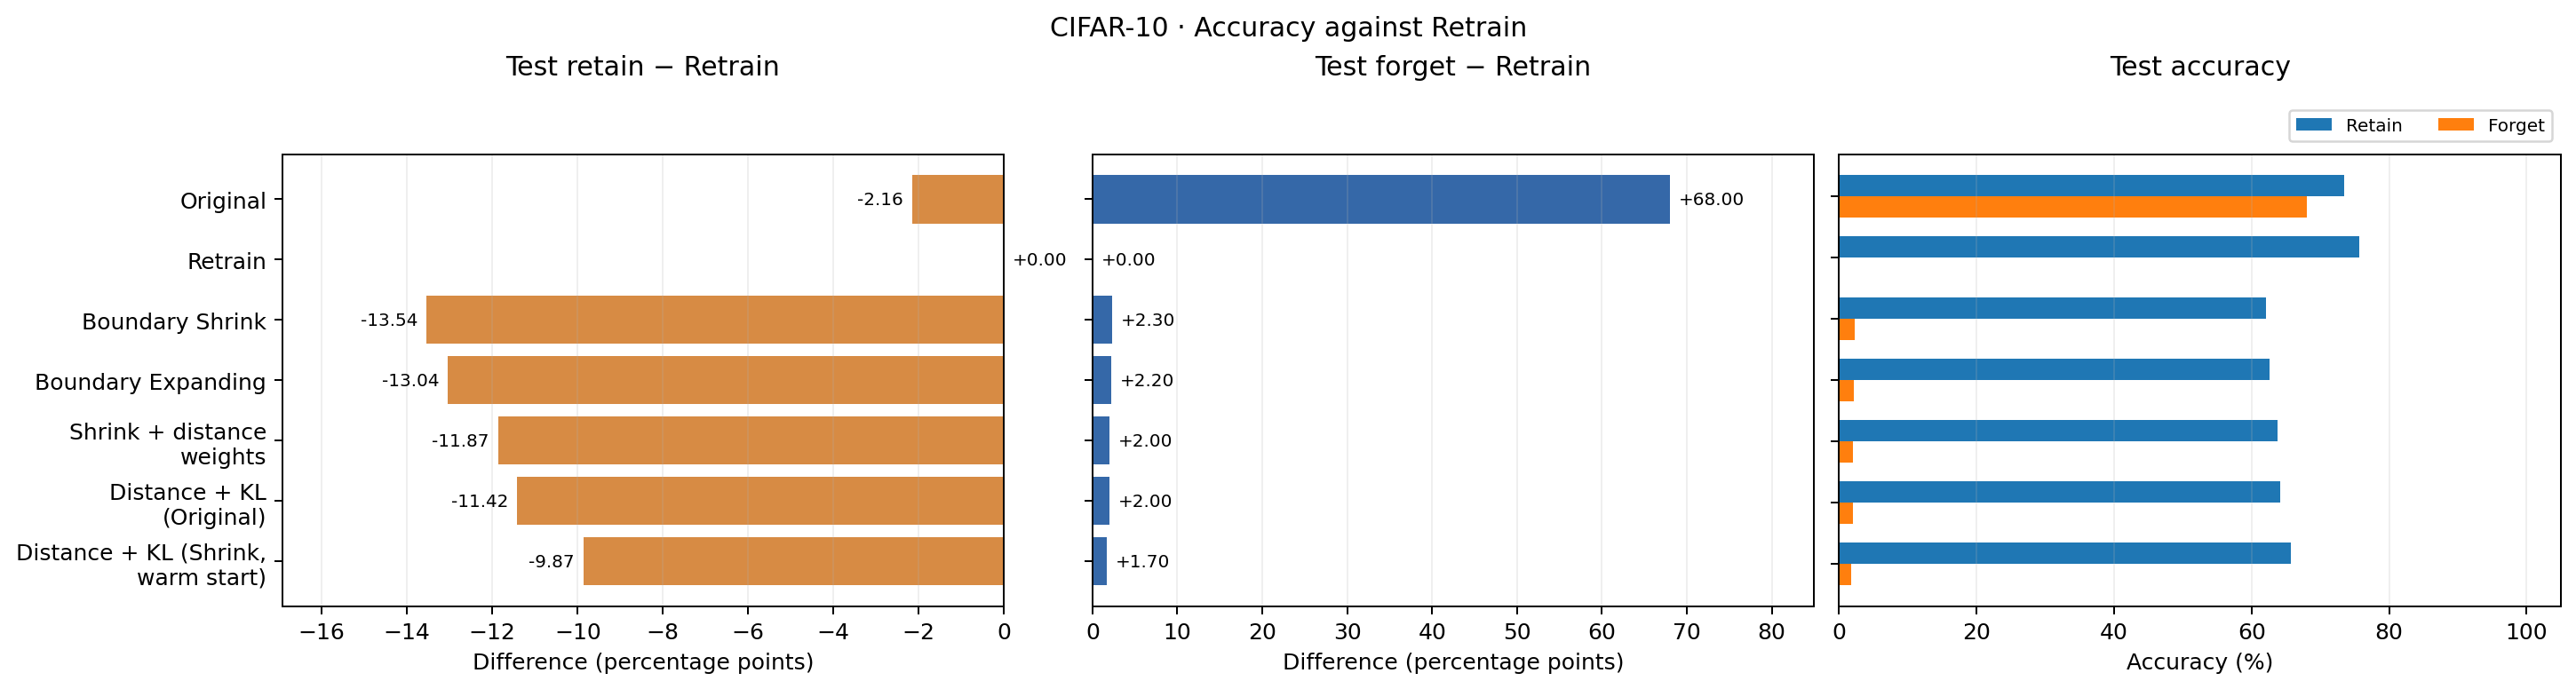
\includegraphics[width=\textwidth]{accuracy.png}
\caption{Độ chính xác kiểm thử và chênh lệch so với Retrain trên CIFAR-10.}
\label{fig:accuracy}
\end{figure*}
\begin{table}[t]
\centering
\caption{Thời gian huấn luyện và unlearning của các mô hình trên CIFAR-10 và CIFAR-100.}
\label{tab:baseline-cost}
\reporttablefont
\setlength{\tabcolsep}{1.5pt}
\renewcommand{\arraystretch}{1.08}
\begin{tabular*}{\columnwidth}{@{\extracolsep{\fill}}>{\raggedright\arraybackslash}p{0.63in}>{\raggedright\arraybackslash}p{0.84in}*{4}{c}@{}}
\toprule
Dataset & Mô hình & \shortstack{Train\\(s)} & \shortstack{Unlearn\\(s)} & \shortstack{Bước\\unlearn} & Tăng tốc \\
\midrule
CIFAR-10 & Original & 436.18 & --- & --- & ---\\
& Retrain & 399.03 & --- & --- & 1.00\(\times\)\\
& Boundary Shrink & --- & 23.24 & 790 & 17.2\(\times\)\\
& Boundary Expanding & --- & 12.62 & 790 & 31.6\(\times\)\\
\midrule
CIFAR-100 & Original & 424.77 & --- & --- & ---\\
& Retrain & 424.53 & --- & --- & 1.00\(\times\)\\
& Boundary Shrink & --- & 3.18 & 80 & 133.6\(\times\)\\
& Boundary Expanding & --- & 1.44 & 80 & 294.0\(\times\)\\
\bottomrule
\end{tabular*}
\end{table}
Bảng~\ref{tab:baseline-cost} cho thấy Boundary Expanding nhanh hơn Boundary Shrink trong cả hai lượt, phù hợp việc không tạo ảnh FGSM mỗi batch. Cả hai nhanh hơn huấn luyện lại trong thiết lập đo nhưng đi kèm khoảng cách utility. Các hệ số tăng tốc trên CIFAR-100 được ghi nhận với tập 500 ảnh forget và ngân sách 80 bước cập nhật.

\subsection{Khảo sát các biến thể của Boundary Shrink trên CIFAR-10}
\begin{table}[t]
\centering
\caption{Độ chính xác (\%) trên CIFAR-10 của Boundary Shrink, các biến thể và Retrain.}
\label{tab:variants}
\reporttablefont
\setlength{\tabcolsep}{1.5pt}
\renewcommand{\arraystretch}{1.08}
\begin{tabular*}{\columnwidth}{@{\extracolsep{\fill}}>{\raggedright\arraybackslash}p{0.82in}*{5}{c}@{}}
\toprule
Phương pháp & \shortstack{Train\\ret.} & \shortstack{Train\\forg.} & \shortstack{Test\\ret.} & \shortstack{Test\\forg.} & \shortstack{Delta\\Retrain} \\
\midrule
Retrain & 99.70 & 0.00 & 75.61 & 0.00 & 0.00\\
Boundary Shrink & 94.86 & 11.54 & 62.07 & 2.30 & \(-\)13.54\\
DW & 95.76 & 10.12 & 63.74 & 2.00 & \(-\)11.87\\
DW+KL-S & 96.63 & 9.14 & 65.74 & 1.70 & \(-\)9.87\\
\bottomrule
\end{tabular*}
\end{table}
Bảng~\ref{tab:variants} cho thấy DW tăng test-retain 1.67 điểm so với Boundary Shrink. DW+KL-S có test-retain cao nhất trong các phương pháp unlearning đã khảo sát, tăng 3.67 điểm so với Boundary Shrink. Test-forget giảm từ 2.30\% xuống 1.70\%, tức còn 17/1.000 ảnh deer được nhận diện đúng. Tuy vậy, cấu hình này vẫn kém Retrain 9.87 điểm test-retain và còn train-forget 9.14\%.

\begin{table}[t]
\centering
\caption{Thời gian thực hiện và số bước cập nhật của Boundary Shrink và các biến thể trên CIFAR-10.}
\label{tab:variant-cost}
\reporttablefont
\setlength{\tabcolsep}{1.5pt}
\renewcommand{\arraystretch}{1.08}
\begin{tabular*}{\columnwidth}{@{\extracolsep{\fill}}>{\raggedright\arraybackslash}p{0.70in}*{5}{c}@{}}
\toprule
Phương pháp & \shortstack{Giai đoạn\\cuối (s)} & \shortstack{Toàn quy trình\\(s)} & \shortstack{Bước\\student} & \shortstack{Tổng\\bước} & Tăng tốc \\
\midrule
Boundary Shrink & 23.24 & 23.24 & 790 & 790 & 17.2\(\times\)\\
DW & 94.35 & 94.35 & 790 & 790 & 4.23\(\times\)\\
DW+KL-S & 109.38 & 226.97 & 1.580 & 2.370 & 1.76\(\times\)\\
\bottomrule
\end{tabular*}
\end{table}
Lợi ích accuracy có chi phí đáng kể (Bảng~\ref{tab:variant-cost}). DW sử dụng thời gian gấp khoảng 4.1 lần Boundary Shrink với cùng 790 bước cập nhật, do thực hiện tìm kiếm trên nhiều mức nhiễu. DW+KL-S có thời gian giai đoạn cuối 109.38 giây và tổng thời gian 226.97 giây, bao gồm chi phí chuẩn bị DW và Boundary Shrink. Tăng tốc của cấu hình đạt 65.74\% là $1.76\times$. Boundary Expanding nhanh nhất trong lượt CIFAR-10; DW+KL-S có test-retain cao nhất trong các phương pháp unlearning đã chạy nhưng tốn ngân sách hơn.

\subsection{Phân tích mô tả trên CIFAR-10}
Các hình bổ trợ ở Phụ lục~\ref{app:visual} dùng cùng các mô hình được đánh giá trên CIFAR-10. Grad-CAM dùng bốn mẫu train-forget, chỉ số 355, 2021, 4644 và 1442 trong tập con. Tầng đích là lớp tích chập cuối, logit đích luôn là deer. Xác suất deer giảm mạnh trên các ví dụ sau unlearning. Các bản đồ thể hiện đóng góp của từng vùng ảnh vào logit deer; nhãn dự đoán kèm theo là lớp có xác suất đầu ra cao nhất. Mỗi CAM được chuẩn hóa min--max riêng, biểu diễn vị trí tương đối của các vùng kích hoạt trong từng mô hình. Xác suất trong hình được hiển thị đến một chữ số thập phân.

ECDF entropy dùng 2.000 mẫu cố định mỗi tập train-retain, train-forget và test. Với $H=-\sum_kp_k\ln p_k$, trục hoành là $\ln(\max(H,10^{-16}))$; $H$ tính bằng nats. Đường train-forget dịch sang entropy lớn hơn sau unlearning, tương tự xu hướng Retrain. Tuy nhiên test đa lớp còn train-forget chỉ có deer, nên khác biệt còn chứa ảnh hưởng thành phần lớp.

 t-SNE dùng 1.200 mẫu test, 120 mẫu mỗi lớp, seed 2022, perplexity 30 và 1.000 vòng lặp. Các mẫu deer còn xen lẫn với nhiều lớp ngay trên Original. Embedding được tính riêng cho từng mô hình, tạo ra các hệ tọa độ độc lập. Phân tích định tính tập trung vào cấu trúc lân cận trong từng phép chiếu.

\section{Thảo luận và giới hạn}
Ở cả hai dataset, việc giảm accuracy lớp quên đi kèm suy giảm accuracy trên các lớp giữ lại. Các phương pháp unlearning có chi phí thấp hơn Retrain nhưng cũng có test-retain thấp hơn, cho thấy đánh đổi giữa thời gian thực hiện và khả năng duy trì hiệu năng trên các lớp giữ lại.

Trên CIFAR-10, hai biến thể của Boundary Shrink cải thiện chỉ số so với phương pháp cơ sở trong lần chạy, nhưng đóng góp riêng của từng thành phần chưa được xác định. DW đồng thời thay đổi pseudo-label, chuẩn hóa attack và trọng số; DW+KL-S thay đổi khởi tạo, teacher và ngân sách. Do các yếu tố này thay đổi đồng thời, chênh lệch quan sát được phản ánh hiệu quả của cấu hình tổng thể.

Thực nghiệm sử dụng một seed và một lớp quên trên mỗi dataset. Độ biến động giữa các lần chạy và giữa các lớp quên chưa được khảo sát. Trên CIFAR-100, tập test-forget gồm 100 ảnh nên mỗi ảnh tương ứng một điểm phần trăm accuracy. Nghiên cứu chưa sử dụng tập validation độc lập và chưa đánh giá tính riêng tư bằng tấn công suy luận thành viên (MIA). Phạm vi kết luận do đó giới hạn ở lớp quên, kiến trúc và cấu hình đã khảo sát.

\section{Kết luận}
Báo cáo đánh giá cùng bốn mô hình Original, Retrain, Boundary Shrink và Boundary Expanding trên CIFAR-10 và CIFAR-100. Trong hai thiết lập, Boundary Shrink và Boundary Expanding giảm accuracy lớp quên với chi phí thấp hơn Retrain, đồng thời làm giảm hiệu năng lớp giữ lại. Trong thí nghiệm trên CIFAR-10, hai biến thể của Boundary Shrink cải thiện test-retain so với phương pháp cơ sở; DW+KL-S đạt 65.74\% test-retain và 1.70\% test-forget, tổng thời gian 226.97 giây, tăng tốc $1.76\times$ so với Retrain. DW+KL-S cải thiện độ chính xác trên các lớp giữ lại so với Boundary Shrink nhưng vẫn thấp hơn Retrain và sử dụng nhiều thời gian hơn phương pháp cơ sở.

% Balance the final two-column page using IEEEtran's reference trigger.
\IEEEtriggeratref{2}
\begin{thebibliography}{10}
\bibitem{bourtoule2021machine}
L. Bourtoule \textit{et al.}, ``Machine Unlearning,'' in \textit{IEEE Symposium on Security and Privacy}, 2021. \url{https://arxiv.org/abs/1912.03817}.
\bibitem{chen2023boundary}
M. Chen, W. Gao, G. Liu, K. Peng, and C. Wang, ``Boundary Unlearning: Rapid Forgetting of Deep Networks via Shifting the Decision Boundary,'' in \textit{CVPR}, 2023, pp. 7766--7775.
\bibitem{golatkar2020eternal}
A. Golatkar, A. Achille, and S. Soatto, ``Eternal Sunshine of the Spotless Net: Selective Forgetting in Deep Networks,'' in \textit{CVPR}, 2020.
\bibitem{goodfellow2015explaining}
I. J. Goodfellow, J. Shlens, and C. Szegedy, ``Explaining and Harnessing Adversarial Examples,'' in \textit{ICLR}, 2015. \url{https://arxiv.org/abs/1412.6572}.
\bibitem{springenberg2015allcnn}
J. T. Springenberg, A. Dosovitskiy, T. Brox, and M. Riedmiller, ``Striving for Simplicity: The All Convolutional Net,'' in \textit{ICLR Workshop}, 2015. \url{https://arxiv.org/abs/1412.6806}.
\bibitem{ioffe2015batch}
S. Ioffe and C. Szegedy, ``Batch Normalization: Accelerating Deep Network Training by Reducing Internal Covariate Shift,'' in \textit{ICML}, 2015, pp. 448--456.
\bibitem{hinton2015distilling}
G. Hinton, O. Vinyals, and J. Dean, ``Distilling the Knowledge in a Neural Network,'' arXiv:1503.02531, 2015.
\bibitem{selvaraju2017gradcam}
R. R. Selvaraju \textit{et al.}, ``Grad-CAM: Visual Explanations from Deep Networks via Gradient-Based Localization,'' in \textit{ICCV}, 2017.
\bibitem{maaten2008tsne}
L. van der Maaten and G. Hinton, ``Visualizing Data using t-SNE,'' \textit{Journal of Machine Learning Research}, vol. 9, pp. 2579--2605, 2008.
\bibitem{krizhevsky2009learning}
A. Krizhevsky, ``Learning Multiple Layers of Features from Tiny Images,'' University of Toronto, Technical Report, 2009. Dataset: \url{https://www.cs.toronto.edu/~kriz/cifar.html}.
\end{thebibliography}
\onecolumn
\appendices
\section{Trực quan hóa bổ trợ trên CIFAR-10}
\label{app:visual}
Phụ lục trình bày Grad-CAM, phân phối entropy và t-SNE của các mô hình trên những mẫu CIFAR-10 cố định.
\begin{figure}[!ht]
\centering
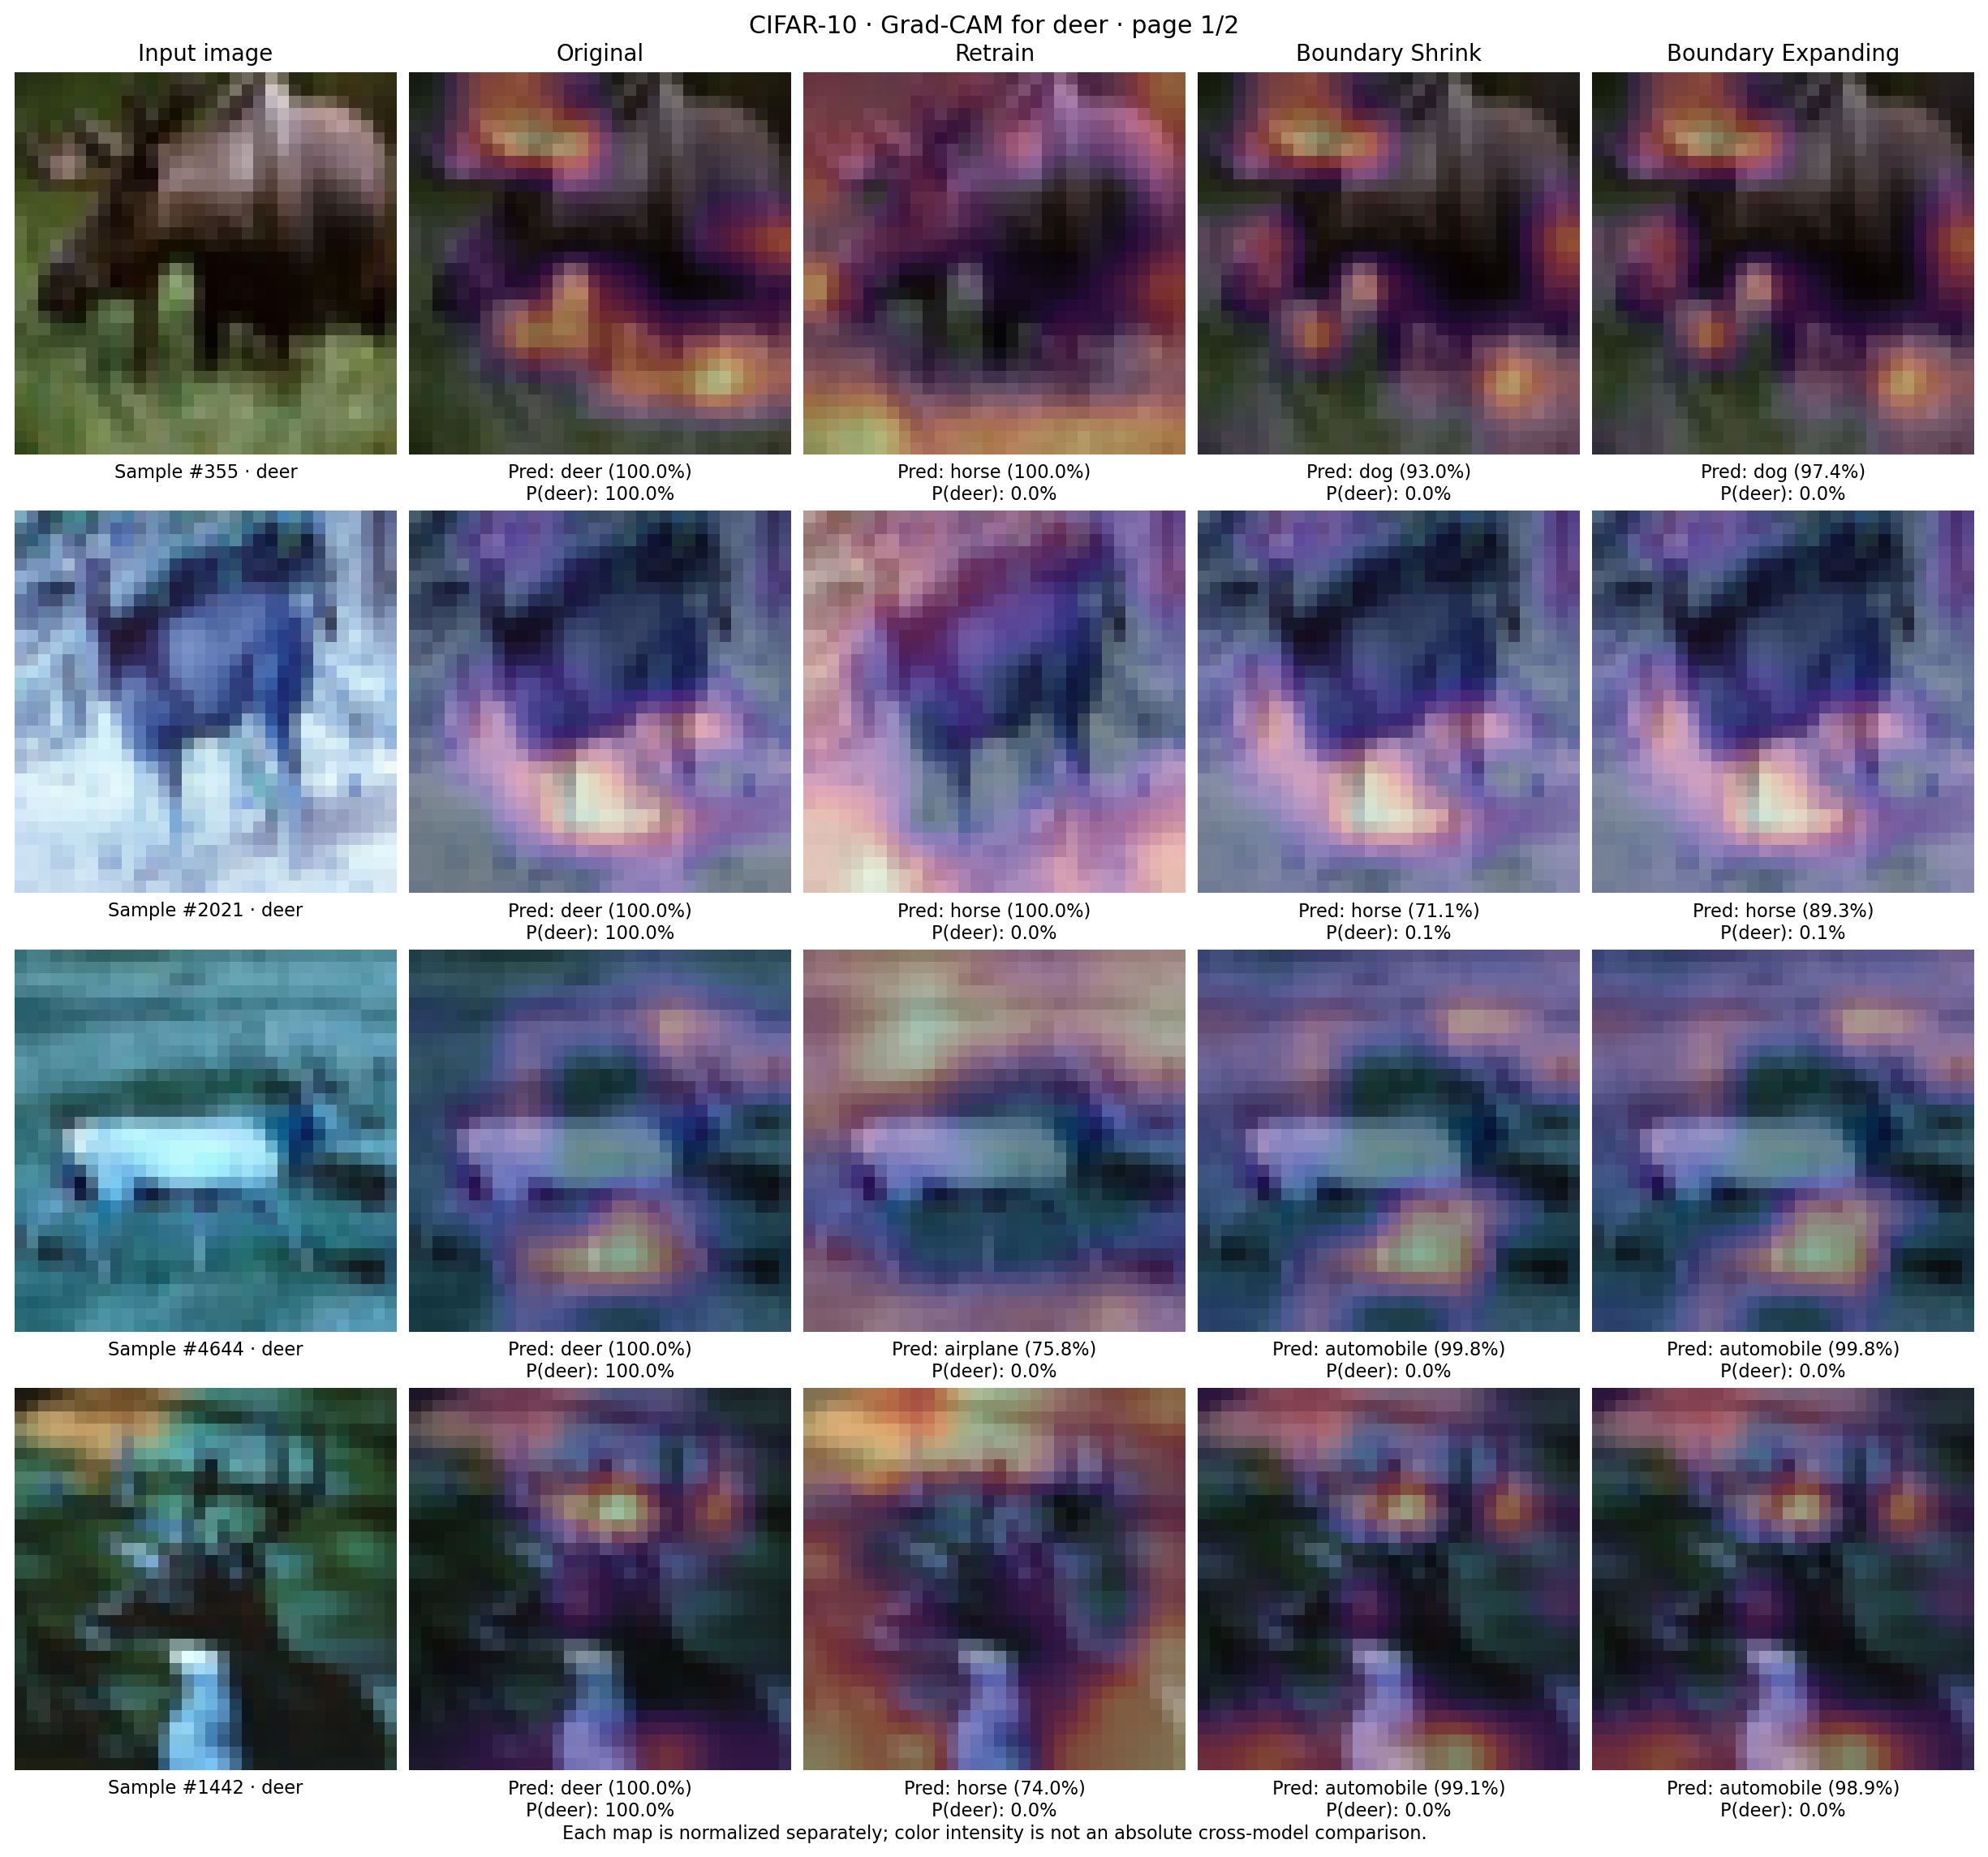
\includegraphics[width=0.94\textwidth,height=0.70\textheight,keepaspectratio]{gradcam_1.png}
\caption{Grad-CAM theo logit deer của Original, Retrain, Boundary Shrink và Boundary Expanding trên bốn mẫu train-forget CIFAR-10.}
\label{fig:cam-base}
\end{figure}
\clearpage
\begin{figure}[!ht]
\centering
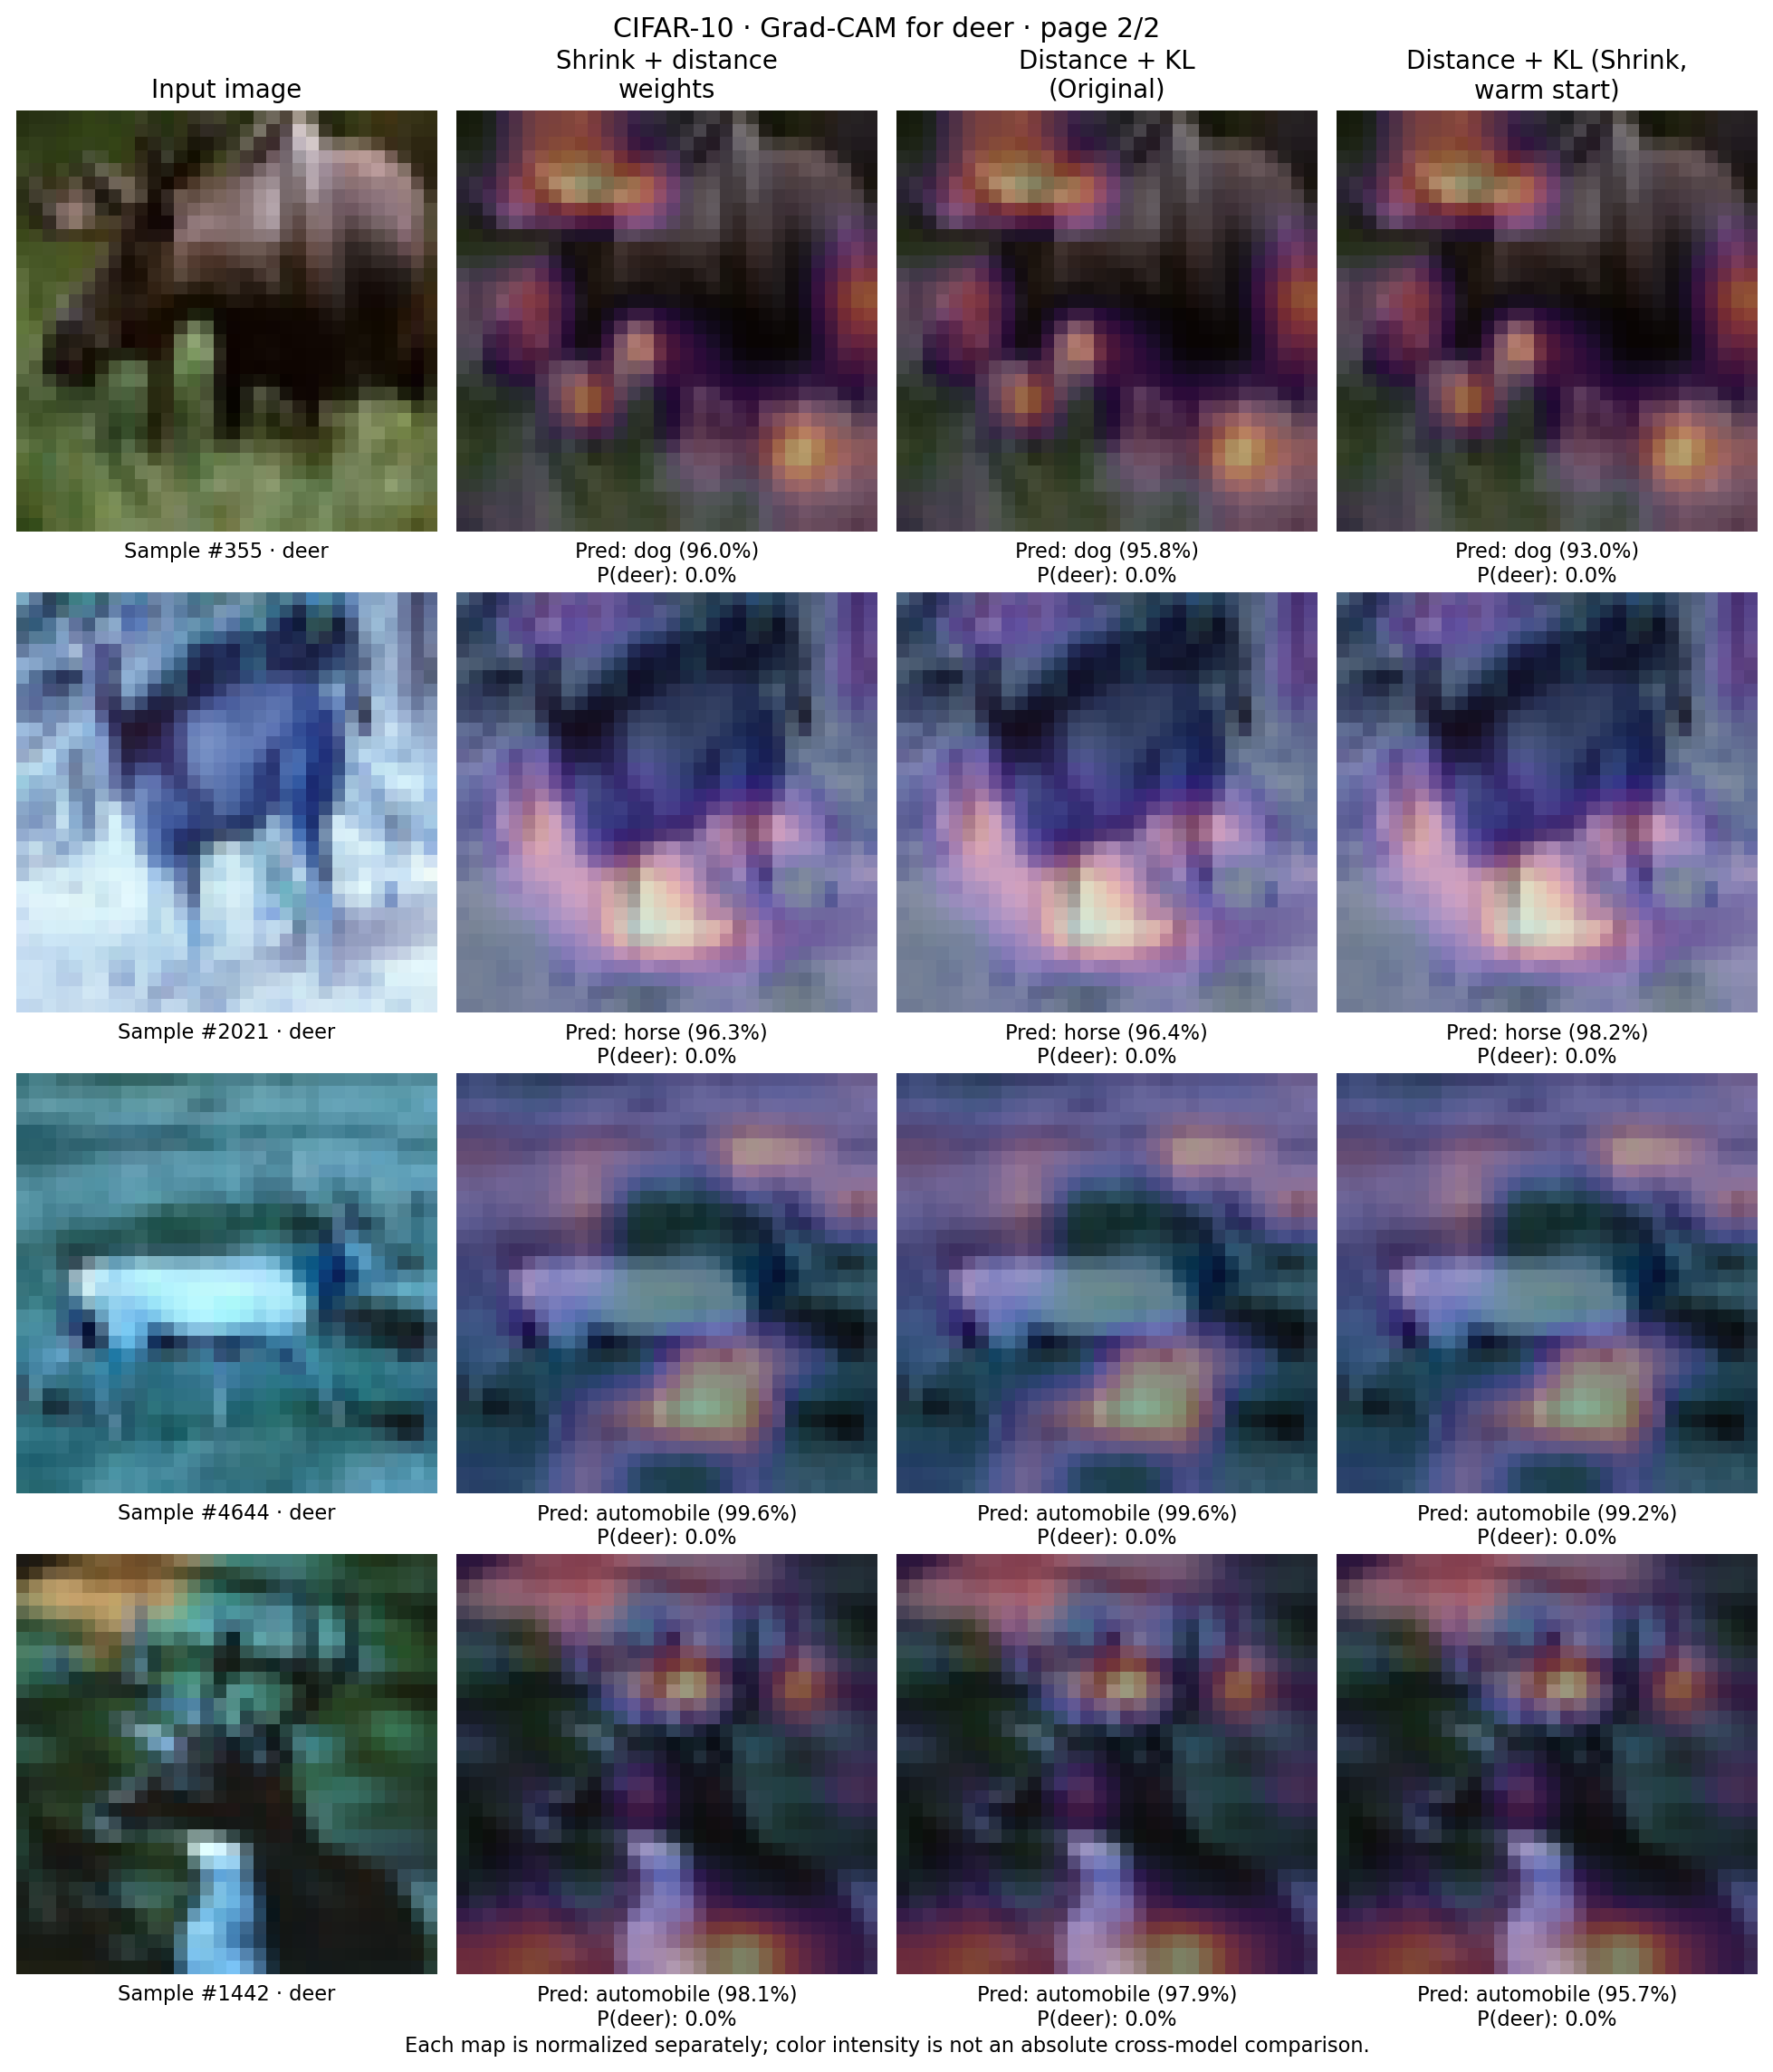
\includegraphics[width=0.84\textwidth,height=0.70\textheight,keepaspectratio]{gradcam_2.png}
\caption{Grad-CAM theo logit deer cho các biến thể của Boundary Shrink trên cùng bốn mẫu train-forget CIFAR-10.}
\label{fig:cam-variants}
\end{figure}
\clearpage
\begin{figure}[!ht]
\centering
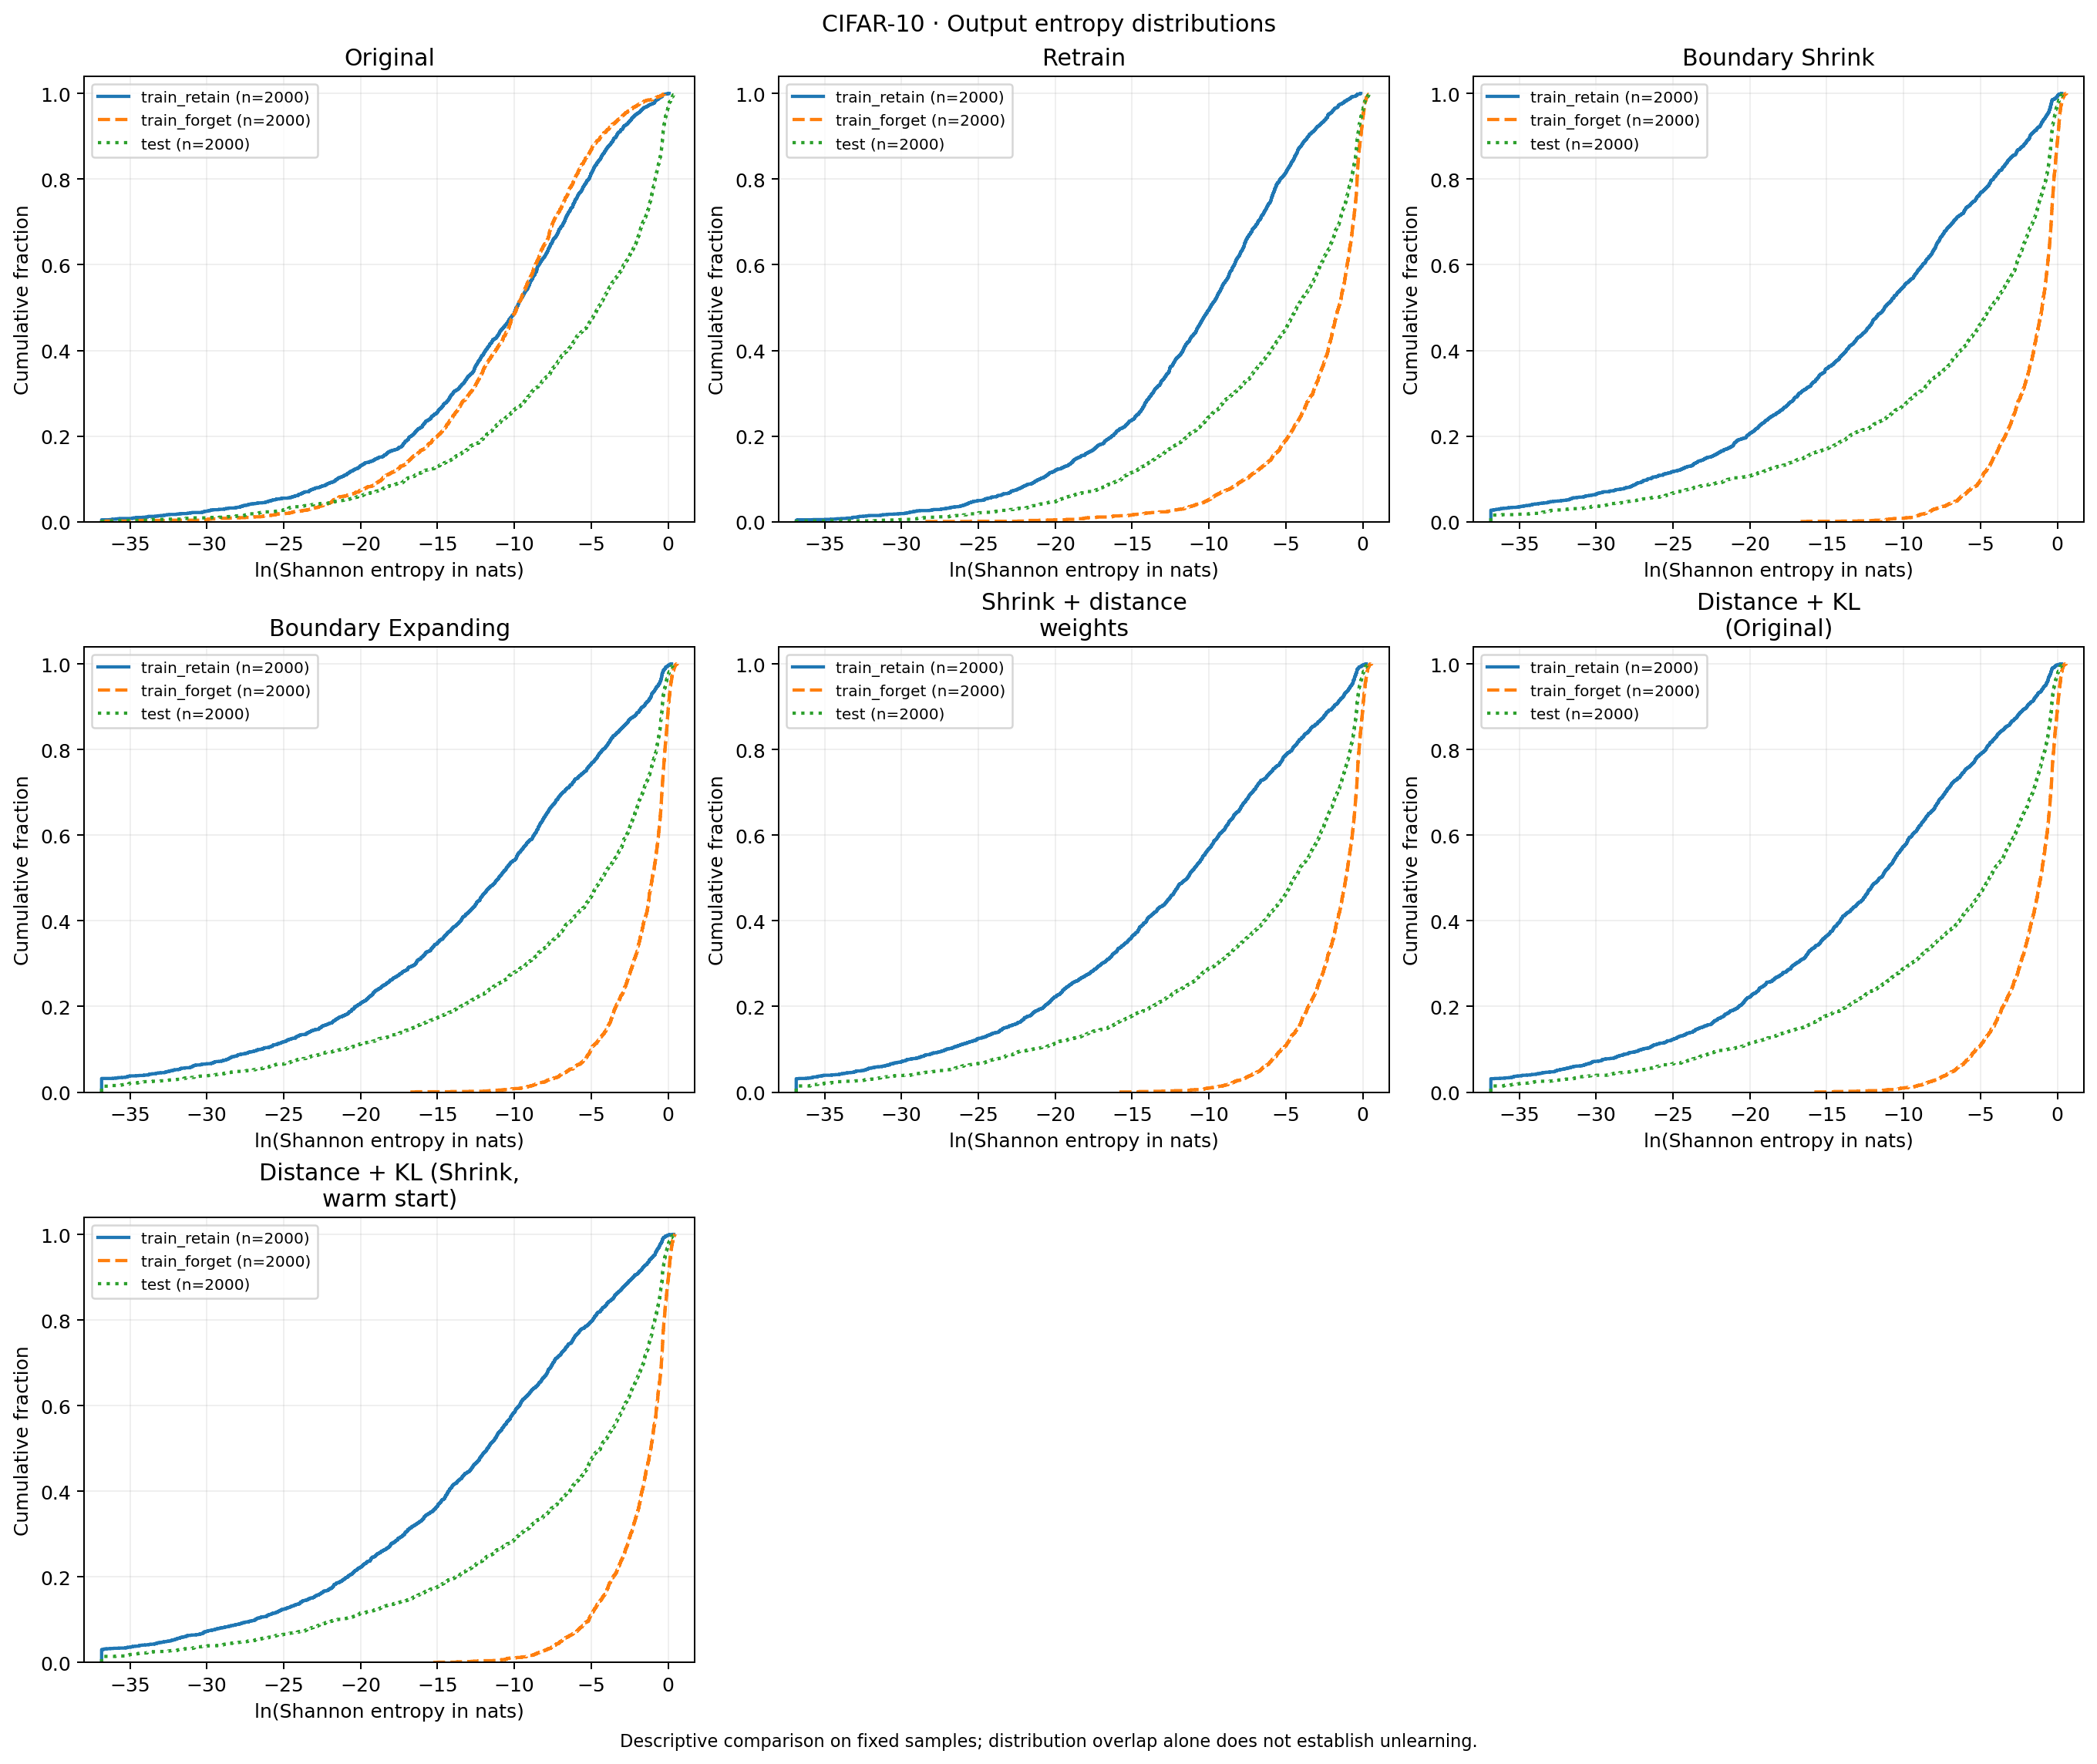
\includegraphics[width=1\textwidth,height=0.76\textheight,keepaspectratio]{entropy.png}
\caption{Phân phối tích lũy thực nghiệm của log entropy trên các tập train-retain, train-forget và test CIFAR-10 (2.000 mẫu mỗi tập).}
\label{fig:entropy}
\end{figure}
\clearpage
\begin{figure}[!ht]
\centering
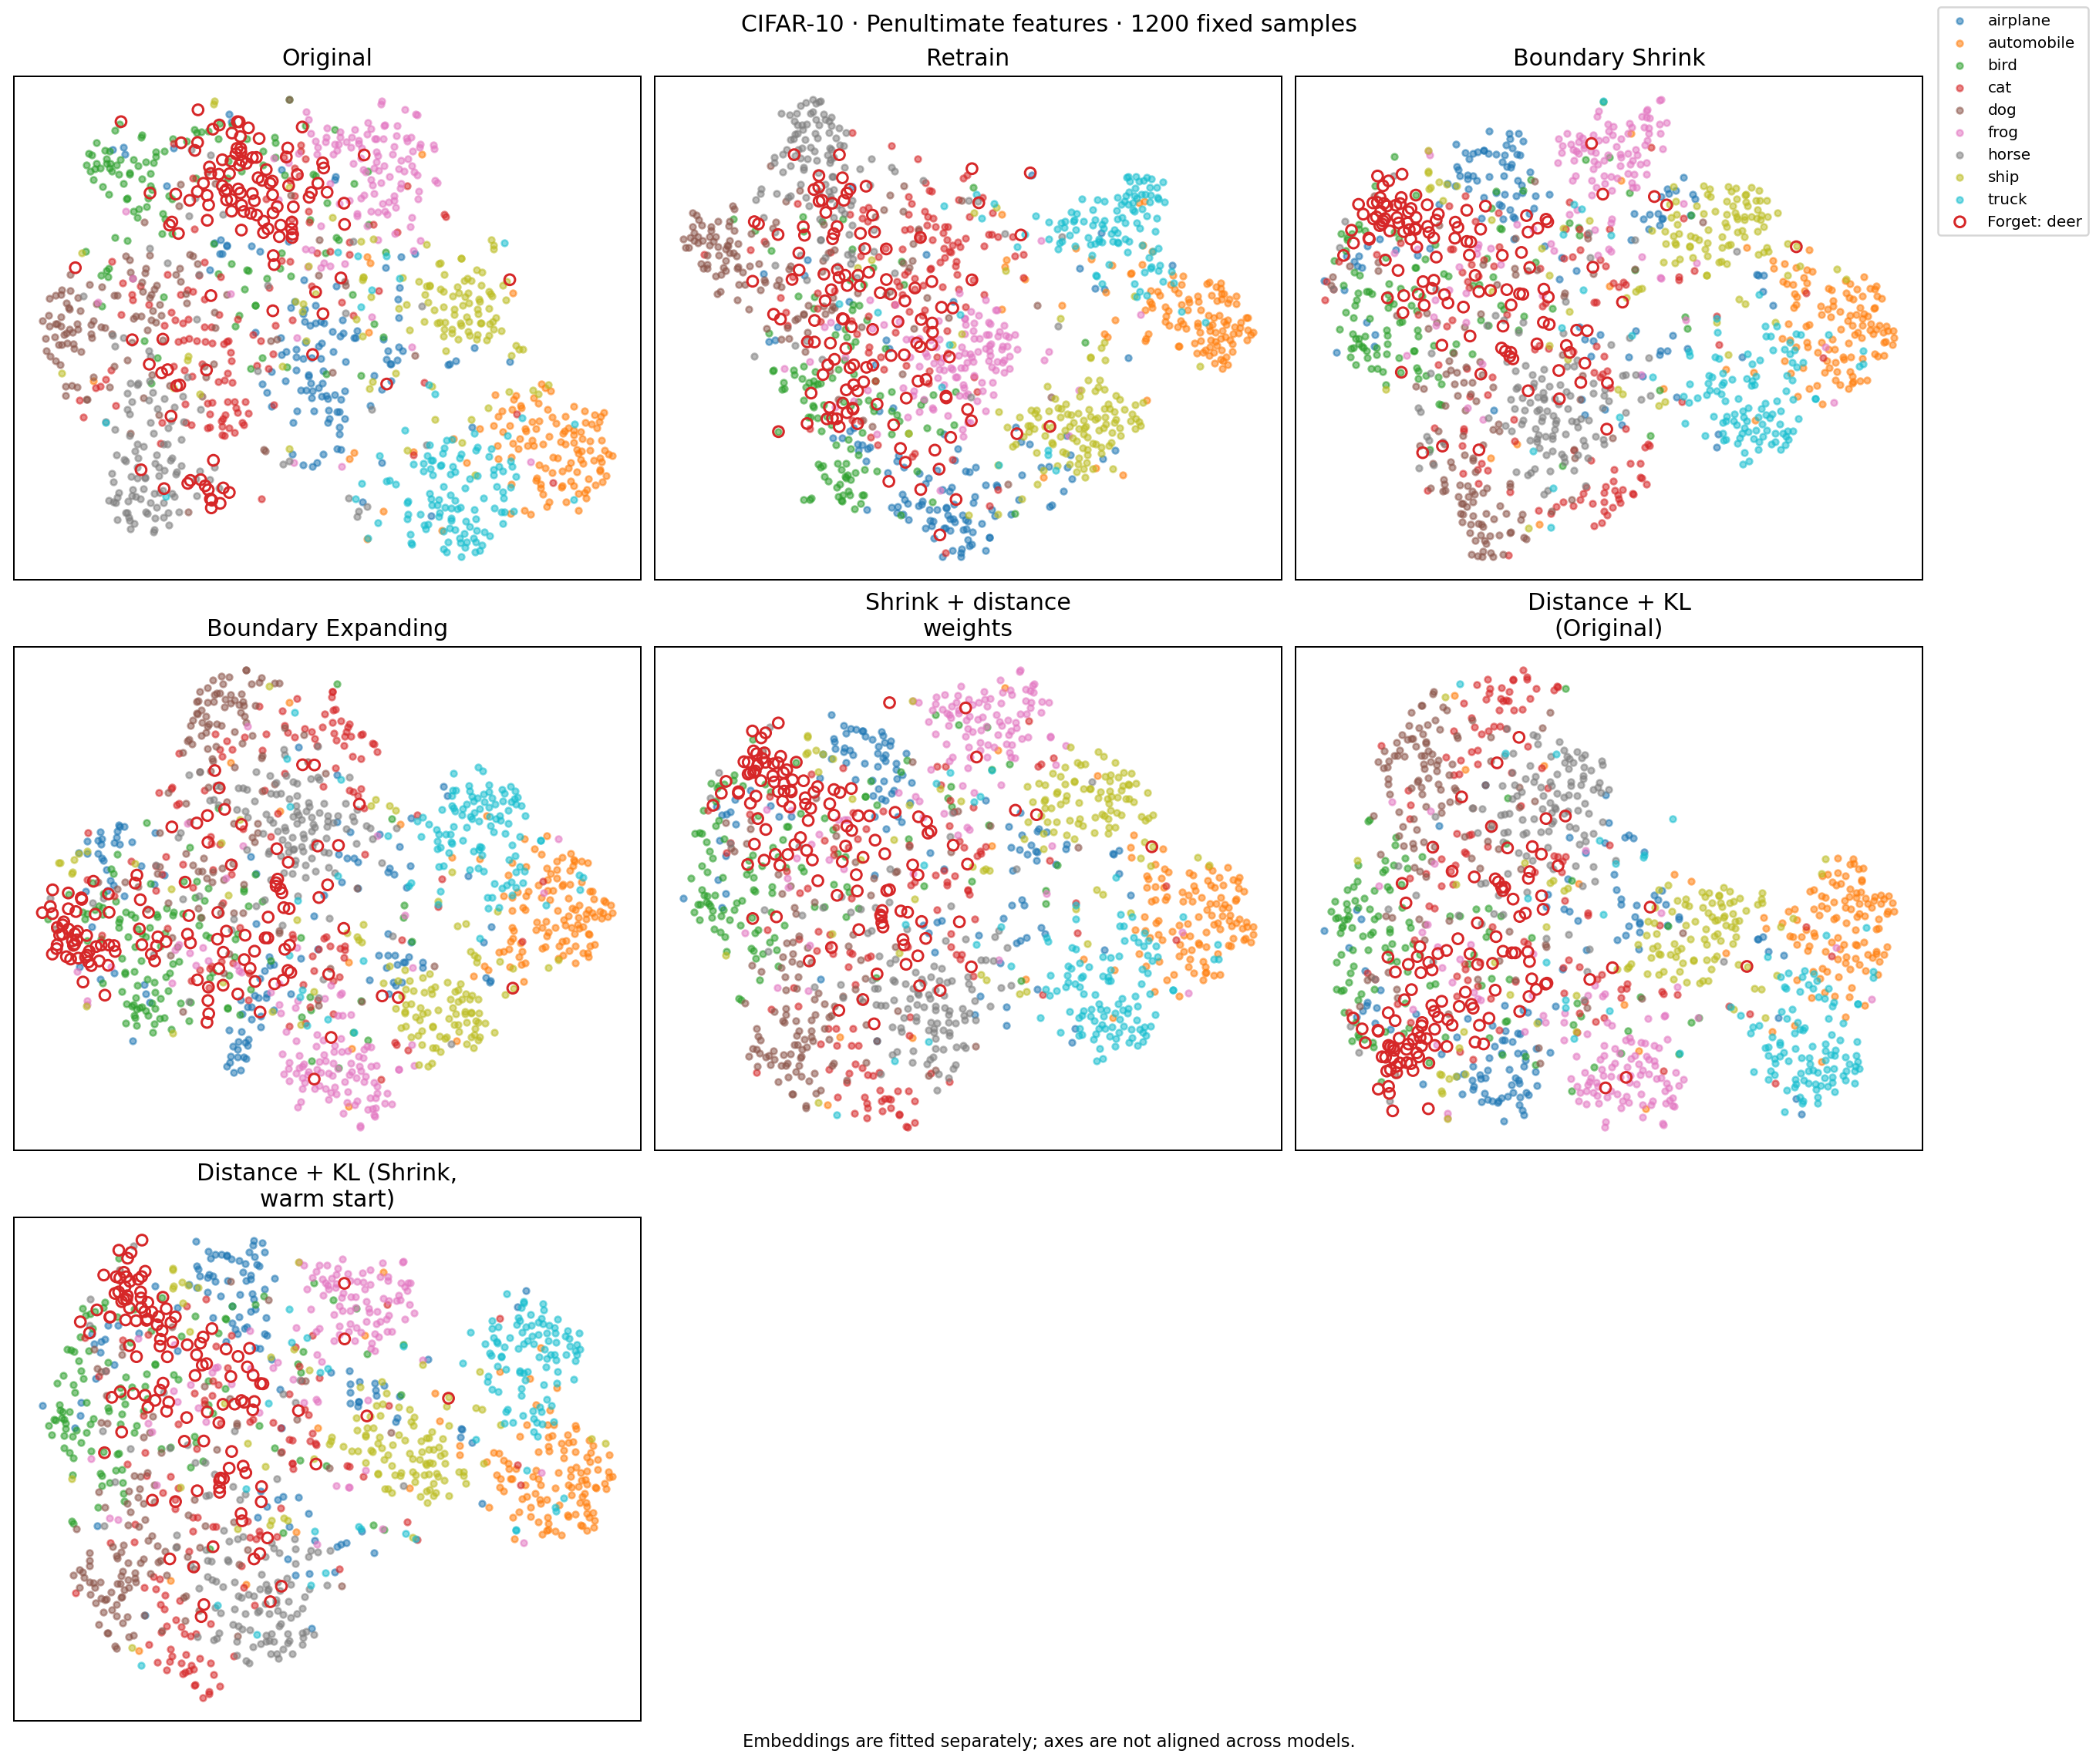
\includegraphics[width=1\textwidth,height=0.76\textheight,keepaspectratio]{tsne.png}
\caption{Biểu diễn t-SNE của 1.200 mẫu kiểm thử CIFAR-10, gồm 120 mẫu mỗi lớp; vòng tròn rỗng biểu thị lớp deer.}
\label{fig:tsne}
\end{figure}
\end{document}
